\section{Introduction}

Information Extraction (IE) is a fundamental task in Natural Language Processing (NLP), which aims to extract structured information from unstructured text~\cite{grishman_2019}, such as Named Entity Recognition (NER), Relation Extraction (RE), Event Extraction (EE), etc.
However, each IE task is usually isolated with specific data structures and delicate models, which makes it difficult to share knowledge across tasks~\cite{uie,genie}.

In order to unify the data formats and take advantage of common features between different tasks, there are two main routes in recent studies.
The first is to utilize generative pretrained language models (PLMs) to generate the structured information directly.
\citet{uie} and \citet{tanl} structure the IE tasks as a sequence-to-sequence problem, and use generative models to predict the structured information autoregressively.
However, such methods cannot provide the exact positions of the structured information, which is important for NER and fair evaluations~\cite{devil-ee}.
Besides, the generation-based methods are usually slow, and it consumes huge resources to train on large-scale datasets~\cite{deepstruct}.
The second is to apply the extractive PLMs, which is way more faster to train and inference.
USM takes the IE tasks into a triplet prediction problems via semantic matching~\cite{usm}.
However, such method is limited in a small range of triplet-based tasks, and not suitable for multi-span and n-ary IE tasks.

\begin{figure}[t]
    \centering
    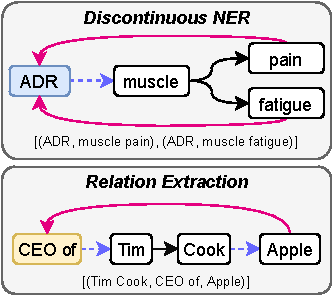
\includegraphics[width=\columnwidth]{figs/Multi-span Cyclic Graph.pdf}
    \caption{
        Multi-span cyclic graph for discontinuous NER and RE tasks (best viewed in color).
        The spans are connected by three types of edges, including \textbf{\textit{consecutive connections}}, dotted \textbf{\color[HTML]{695efb} \textit{jump connections}} and \textbf{\color[HTML]{E9087F} \textit{tail-to-head connections}}.
        \textit{ADR} in discontinuous NER denotes the entity label of Adverse Drug Reaction.
    }
    \label{fig:multi-span-cyclic-graph}
\end{figure}

\begin{table*}[t]
    \centering
    % \resizebox{\textwidth}{!}{%
        \begin{tabular}{c|ccccc|c}
        \toprule
        Model       & TANL    & UIE      & DeepStruct & InstructUIE & USM        & Mirror \\
        \midrule
        PLM         & T5-base & T5-large & GLM        & FlanT5 & RoBERTa    & DeBERTa-v3 \\
        \#Params    & 220M    & 770M     & 10B        & 11B & large 372M & large 434M \\
        \midrule
        % Single-step & {\color[HTML]{008114}\cmark}    & {\color[HTML]{008114}\cmark}   & {\color[HTML]{008114}\cmark} & {\color[HTML]{008114}\cmark} & {\color[HTML]{008114}\cmark} \\
        % NAR         & \textcolor{red}{\xmark}         & \textcolor{red}{\xmark}        & \textcolor{red}{\xmark}      & {\color[HTML]{008114}\cmark} & {\color[HTML]{008114}\cmark} \\
        Decoding    & AR                      & AR                      & AR                      & AR                      & NAR                          & NAR                          \\
        Indexing    & \textcolor{red}{\xmark} & \textcolor{red}{\xmark} & \textcolor{red}{\xmark} & \textcolor{red}{\xmark} & {\color[HTML]{008114}\cmark} & {\color[HTML]{008114}\cmark} \\
        \midrule
        Triplet     & {\color[HTML]{008114}\cmark} & {\color[HTML]{008114}\cmark} & {\color[HTML]{008114}\cmark} & {\color[HTML]{008114}\cmark} & {\color[HTML]{008114}\cmark} & {\color[HTML]{008114}\cmark} \\
        Single-span NER & {\color[HTML]{008114}\cmark} & {\color[HTML]{008114}\cmark} & {\color[HTML]{008114}\cmark} & {\color[HTML]{008114}\cmark} & {\color[HTML]{008114}\cmark} & {\color[HTML]{008114}\cmark} \\
        Multi-span  & \textcolor{red}{\xmark} & $\circ$                 & $\circ$                 & $\circ$                 & \textcolor{red}{\xmark} & {\color[HTML]{008114}\cmark} \\
        N-ary       & \textcolor{red}{\xmark} & \textcolor{red}{\xmark} & \textcolor{red}{\xmark} & \textcolor{red}{\xmark} & \textcolor{red}{\xmark} & {\color[HTML]{008114}\cmark} \\
        Cls.        & \textcolor{red}{\xmark} & \textcolor{red}{\xmark} & \textcolor{red}{\xmark} & $\circ$                 & \textcolor{red}{\xmark} & {\color[HTML]{008114}\cmark} \\
        MRC         & \textcolor{red}{\xmark} & \textcolor{red}{\xmark} & \textcolor{red}{\xmark} & \textcolor{red}{\xmark} & $\circ$                 & {\color[HTML]{008114}\cmark} \\
        \bottomrule
        \end{tabular}
    % }
    \caption{
        Comparisons with other systems.
        % Single-step represents that the model predicts results in a single step.
        \textbf{Circle} $\circ$ indicates the model supports the task theoretically, but the implementation is not available.
        \textbf{AR} denotes the auto-regressive decoding while \textbf{NAR} is the non-autoregressive decoding strategy.
        \textbf{Indexing} means whether the model could provide exact information positions.
        \textbf{Triplet} stands for ``(head, relation, tail)'' triplet extraction.
        \textbf{Single-span NER} denotes flat, and nested NER tasks with consecutive spans.
        \textbf{Multi-span} means the model supports multi-span extraction, e.g. the discontinuous named entity recognition task.
        \textbf{N-ary} denotes the ability of n-ary tuple extraction, e.g. quadruple extraction.
        \textbf{Cls.} represents the classfication and multi-choice Machine Reading Comprehension (MRC) support.
        \textbf{MRC} stands for extractive Question Answering (QA) and extractive MRC task support.
    }
    \label{tab:method_comparison}
\end{table*}

% \begin{table*}[t]
%     \centering
%     \resizebox{\textwidth}{!}{%
%         \begin{tabular}{c|ccccccc|c}
%         \toprule
%         Model & TANL & UIE & DeepStruct & InstructUIE & USM & UniEX & RexUIE & Mirror \\
%         \midrule
%         PLM & T5-base & T5-large & GLM & FlanT5 & RoBERTa & RoBERTa & DeBERTa-v3 & DeBERTa-v3 \\
%         \#Params & 220M & 770M & 10B & 11B & large 372M & large 372M & large 434M & large 434M \\
%         \midrule
%         Single-step & {\color[HTML]{008114}\cmark}    & {\color[HTML]{008114}\cmark}   & {\color[HTML]{008114}\cmark}          & {\color[HTML]{008114}\cmark}           & {\color[HTML]{008114}\cmark}   & {\color[HTML]{008114}\cmark}     & \textcolor{red}{\xmark}      & {\color[HTML]{008114}\cmark}      \\
%         Indexing & \textcolor{red}{\xmark} & \textcolor{red}{\xmark} & \textcolor{red}{\xmark} & \textcolor{red}{\xmark} & {\color[HTML]{008114}\cmark} & {\color[HTML]{008114}\cmark} & {\color[HTML]{008114}\cmark} & {\color[HTML]{008114}\cmark} \\
%         NAR         & \textcolor{red}{\xmark}    & \textcolor{red}{\xmark}   & \textcolor{red}{\xmark}          & \textcolor{red}{\xmark}           & {\color[HTML]{008114}\cmark}   & {\color[HTML]{008114}\cmark}     & {\color[HTML]{008114}\cmark}      & {\color[HTML]{008114}\cmark}      \\
%         Multi-span  & \textcolor{red}{\xmark}    & $\circ$    & $\circ$           & $\circ$            & \textcolor{red}{\xmark}   & \textcolor{red}{\xmark}     & \textcolor{red}{\xmark}      & {\color[HTML]{008114}\cmark}      \\
%         N-ary       & \textcolor{red}{\xmark}    & \textcolor{red}{\xmark}   & \textcolor{red}{\xmark}          & \textcolor{red}{\xmark}           & \textcolor{red}{\xmark}   & \textcolor{red}{\xmark}     & {\color[HTML]{008114}\cmark}      & {\color[HTML]{008114}\cmark} \\
%         \bottomrule
%         \end{tabular}
%     }
%     \caption{
%         Comparisons with other systems.
%         Single-step represents that the model predicts results in a single step.
%         Indexing means whether the model could provide exact information positions.
%         NAR denotes the non-autoregressive decoding strategy.
%         Multi-span means the model supports multi-span extraction, e.g. the discontinuous named entity recognition task.
%         N-ary denotes the ability of n-ary tuple extraction.
%         $\circ$ means the model supports the task theoretically, but the implementation is not available.
%     }
%     \label{tab:method_comparison}
% \end{table*}

To extend the universal IE system into more tasks, we propose \textit{Mirror}, a new IE framework that can be applied in multi-span extraction, n-ary extraction, machine reading comprehension (MRC) and even classification tasks.
As examplified in Figure~\ref{fig:multi-span-cyclic-graph}, we formulate IE tasks into a unified multi-slot tuple extraction problem, and transform those tuples into multi-span cyclic graphs.
This graph structure is rather flexible and scalable.
It can be applied to span-only MRC tasks, label-only classification tasks, and label-span mixed IE tasks.
Mirror takes schemas as part of the model inputs, and this benefits few-shot and zero-shot tasks naturally.

% how well did we do it
We conduct extensive experiments on 30 datasets from 8 tasks, including NER, RE, EE, Aspect-based Sentiment Analysis (ABSA), multi-span discontinuous NER, n-ary hyper RE, MRC and classfication.
To enhance the few-shot and zero-shot abilities, we manually collect 57 datasets into a whole corpus for model pretraining.
Our Mirror shows good compatibility across different tasks and datasets, and achieves competitive results on few-shot and zero-shot settings.

% contribution
Our contributions are summarized as follows:
\begin{itemize}
    \item We propose a unified schema-guided multi-slot extraction paradigm, which is capable of span-only MRC, label-only classification and label-span mixed information extraction tasks.
    \item We propose Mirror, a universal non-autoregressive framework that transforms multiple tasks into a multi-span cyclic graph.
    \item We conduct extensive experiments on 30 datasets from 8 tasks, and the results show that our model achieves competitive results on single-tasks, and outperforms previous SOTA systems on few-shot and zero-shot settings.
\end{itemize}
